\chapter{Model Validation and Simulation}
\label{ch:model}

The model attempts to recreate a microgrid which uses some form of DER as a primary power source along side energy storage in order power the load. \autoref{fig:abridged_flow_diagram} shows a simplified flow diagram of the model using an ORC for the DER. The components include a ORC as a source, a load, a form of energy storage, and an inverter to link the energy storage with other pieces. The ORC block is made up of heat exchangers, an isentropic pump, an isentropic exapnder, and an induction generator. The load block \verb|one line description of load|. The energy storage block \verb|one line description of energy storage|. The inverter block \verb|one line description of inverter|.

\begin{figure}[h]
	\centering
	\caption{A simplified diagram of power and data flows of the model. Blue lines represent electrical power connections and flows similar to a one-line diagram. Green boxes represent data flow from one part of the model to another.}
	\label{fig:abridged_flow_diagram_label}
	
	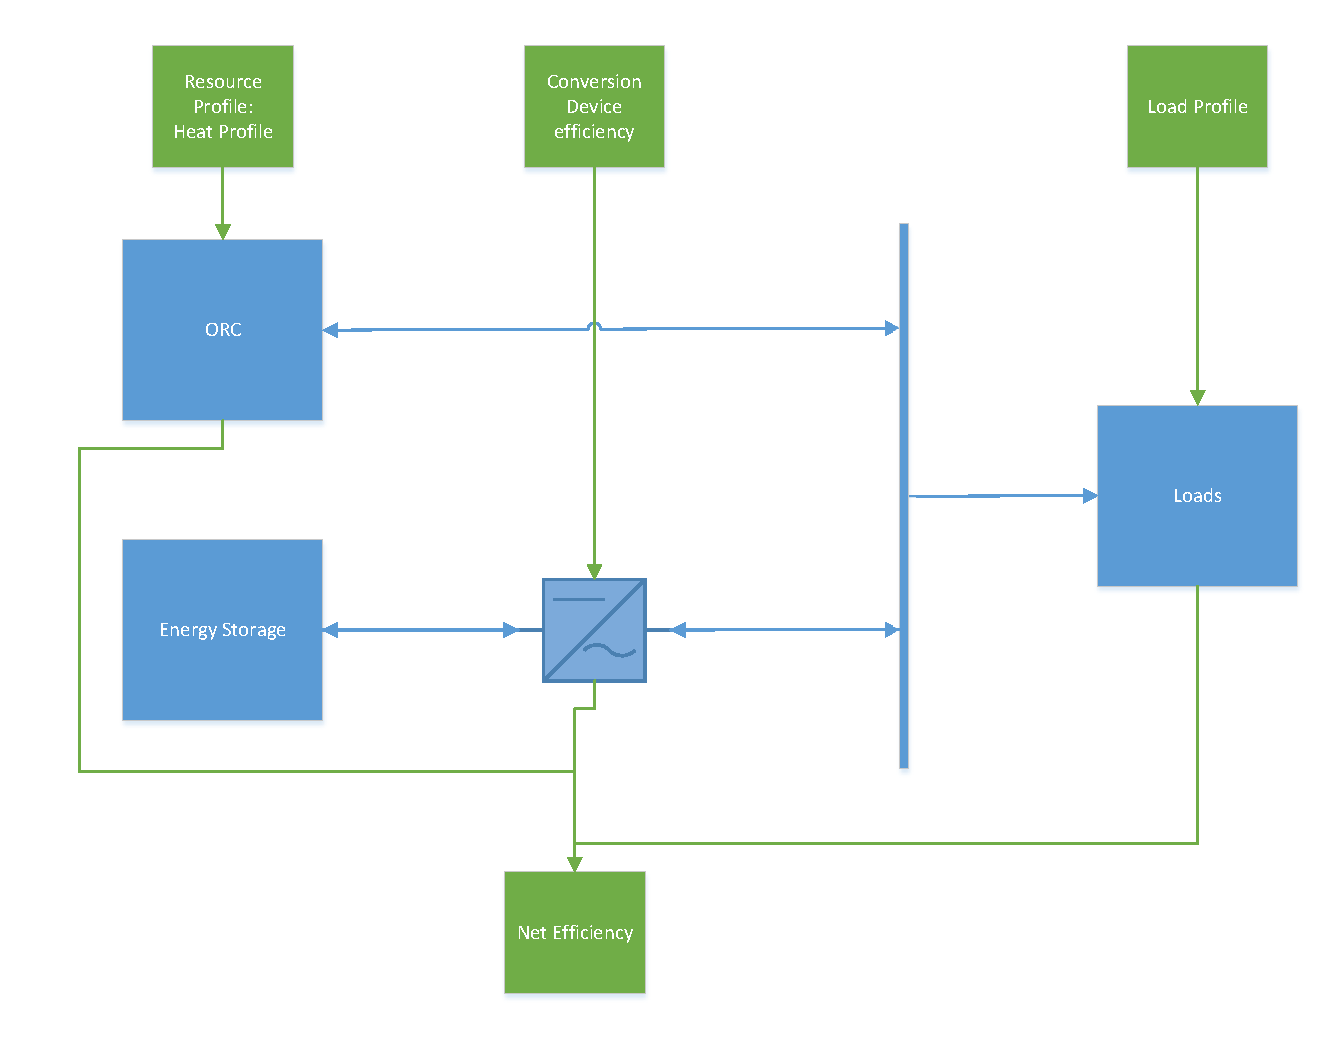
\includegraphics[width=\textwidth]{figures/Abridged Pilgrim Model Flow diagram - AC bus.pdf} 
	%\includegraphics[width=\textwidth]{figures/SimpleFlowDiagram.pdf}

\end{figure}